\begin{figure*} 
\begin{subfigure}[t]{0.10\linewidth}
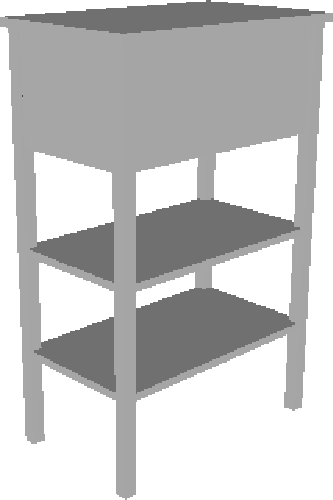
\includegraphics[width=0.9\linewidth]{images/table1_gt.pdf}
\end{subfigure}
\begin{subfigure}[t]{0.098\linewidth}
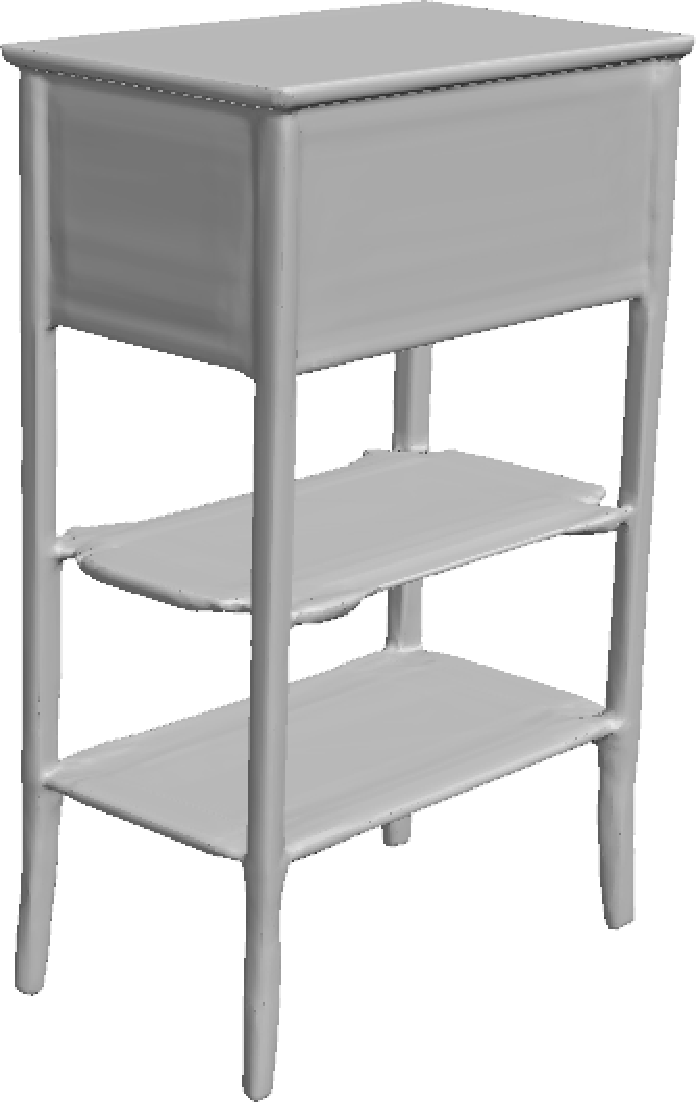
\includegraphics[width=0.9\linewidth]{images/table1_ours.pdf}
\end{subfigure}
\hfill
\begin{subfigure}[t]{0.135\linewidth}
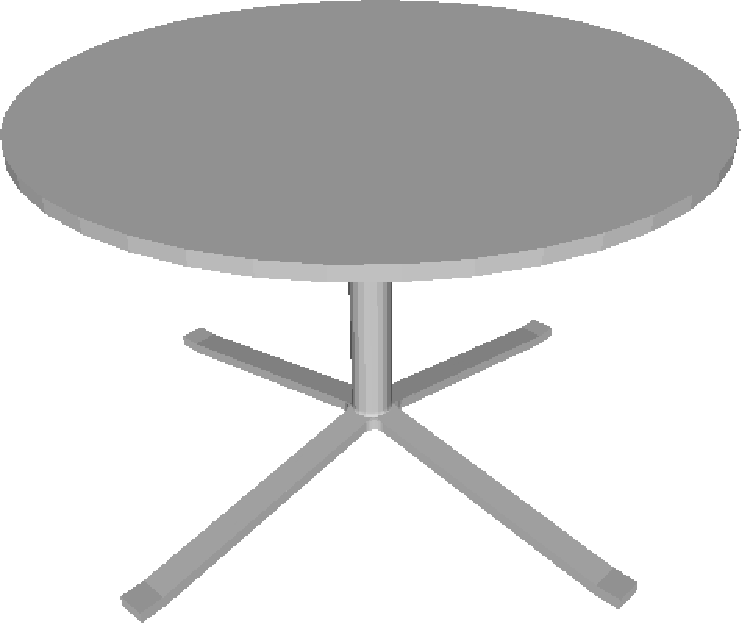
\includegraphics[width=0.9\linewidth]{images/table_gt2.pdf}
\end{subfigure}
\begin{subfigure}[t]{0.13\linewidth}
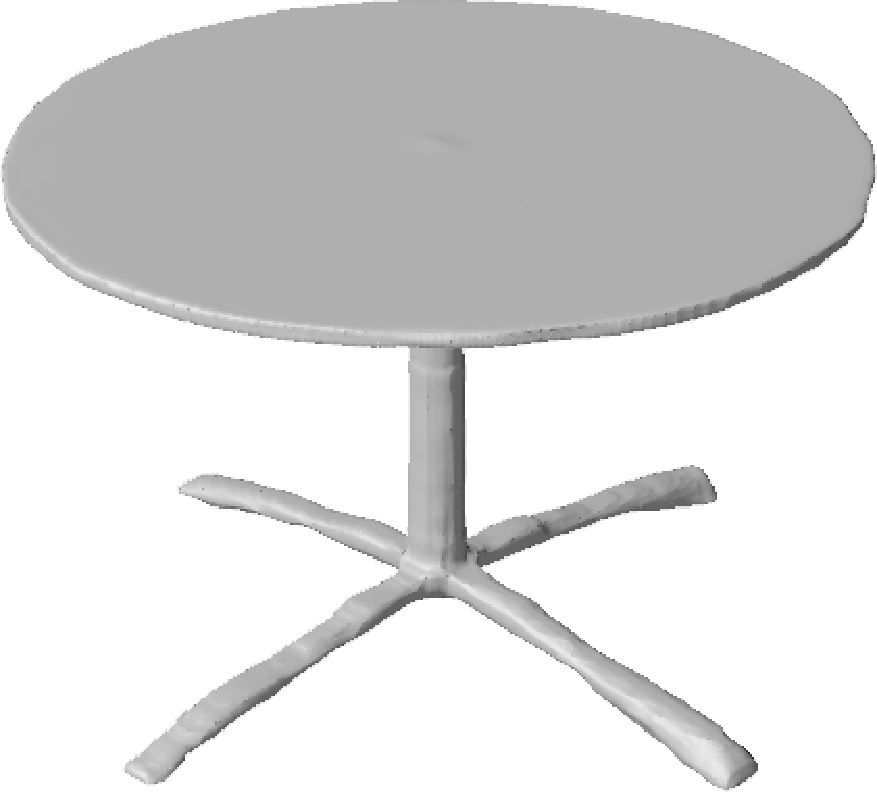
\includegraphics[width=0.9\linewidth]{images/table2_ours.pdf}
\end{subfigure}
\hfill
\begin{subfigure}[t]{0.14\linewidth}
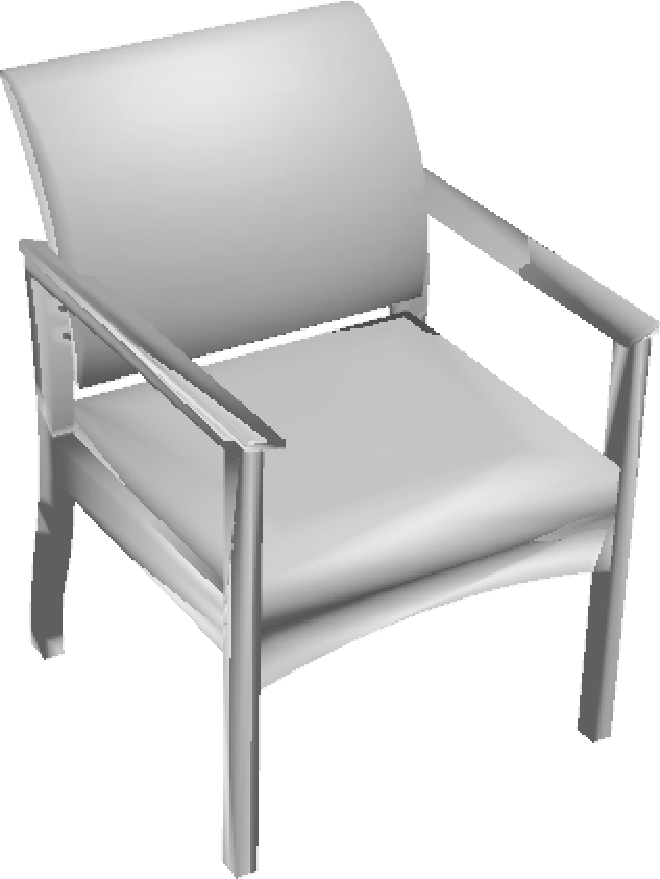
\includegraphics[width=0.9\linewidth]{images/chair2-gt.pdf}
\end{subfigure}
\begin{subfigure}[t]{0.14\linewidth}
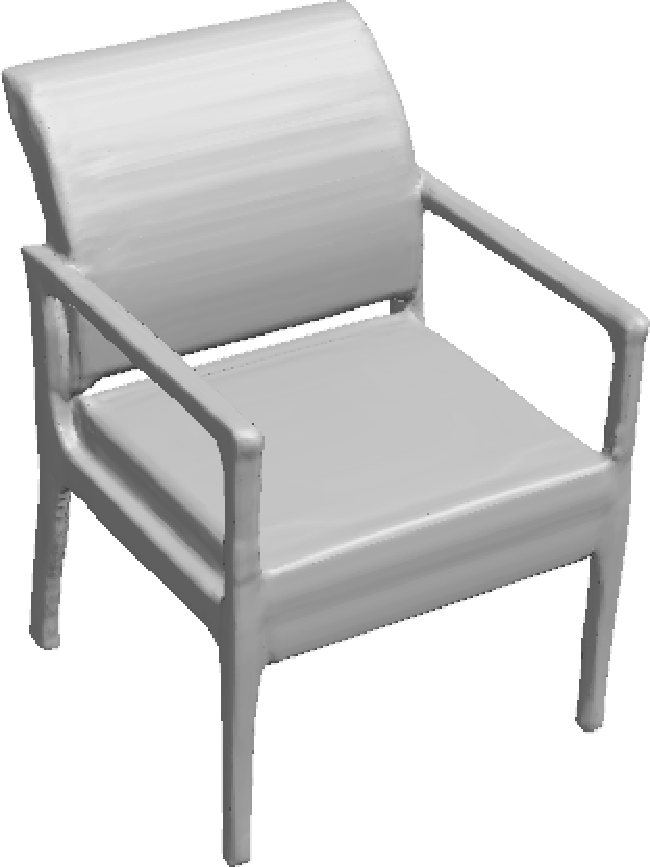
\includegraphics[width=0.9\linewidth]{images/chair2-ours.pdf}
\end{subfigure}
\hfill
\rulesep
\hfill
\begin{subfigure}[t]{0.13\linewidth}
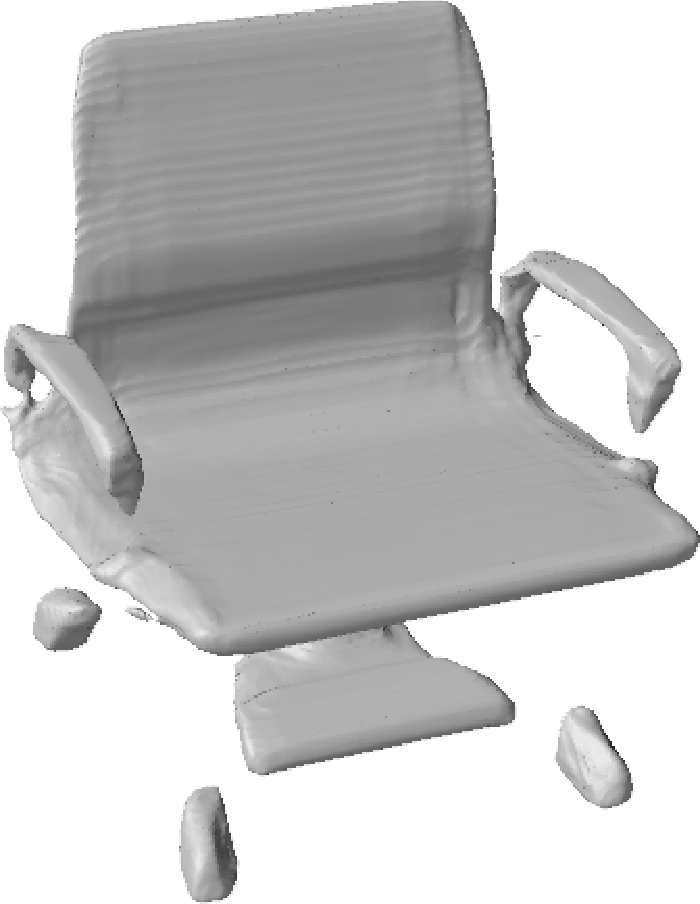
\includegraphics[width=0.9\linewidth]{images/failure1.pdf}
\end{subfigure}
\begin{subfigure}[t]{0.08\linewidth}
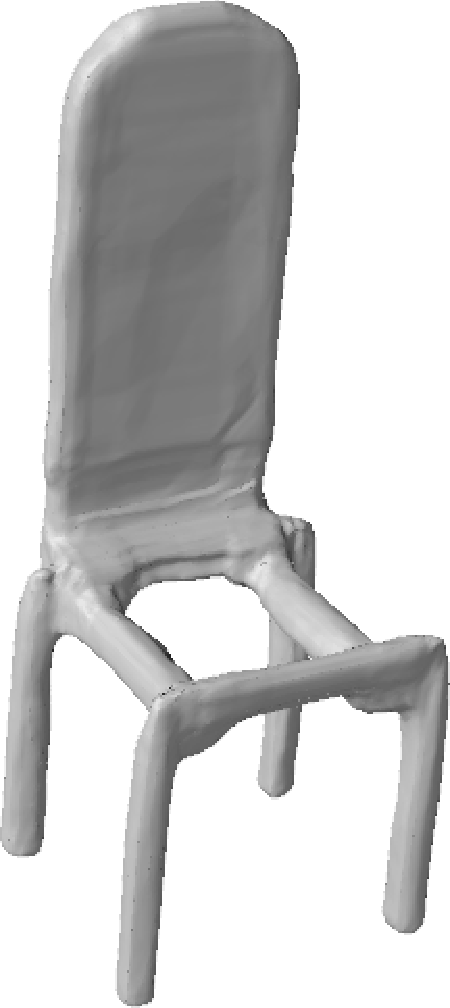
\includegraphics[width=0.9\linewidth]{images/failture2.pdf}
\end{subfigure}
\caption{Reconstruction of test shapes. From left to right alternating: ground truth shape and our reconstruction. The two right most columns show failure modes of DeepSDF. These failures are likely due to lack of training data and failure of minimization convergence.} 
	\label{fig: reconstruction}
\end{figure*}